\documentclass[aspectratio=169, table, 12pt]{beamer}

\usepackage{colortbl}
\usepackage{xcolor}
\usepackage{listings}
\usepackage{tabularx}
\usepackage{tikz}
\usetikzlibrary{arrows.meta, positioning, calc, fit, shapes.geometric}

\makeatletter
\def\input@path{{../theme/}}
\makeatother
\graphicspath{{../theme/}{../../figures/}}
\usetheme{Pradita}

\definecolor{praditagreen}{RGB}{37, 113, 71}

% Tema membuat garis tabel berwarna putih. Dikembalikan agar tabel terbaca.
\arrayrulecolor{black}
\setlength{\arrayrulewidth}{0.5pt}

% Menempatkan gambar di tengah kolom, mendatar sekaligus tegak. Lebarnya
% dipenuhi selebar kolom. Bila hasilnya melebihi tinggi yang disediakan,
% tingginya yang menjadi pembatas, sehingga gambar tidak menembus bingkai.
\newsavebox{\kotakkolom}
\newcommand{\gambarkolom}[2][0.72\textheight]{%
  \sbox{\kotakkolom}{\resizebox{\linewidth}{!}{#2}}%
  \begin{minipage}[c][#1][c]{\linewidth}%
    \centering
    \ifdim\dimexpr\ht\kotakkolom+\dp\kotakkolom\relax>#1\relax
      \resizebox{!}{#1}{#2}%
    \else
      \usebox{\kotakkolom}%
    \fi
  \end{minipage}%
}

\lstdefinestyle{PythonStyle}{
  language=Python,
  basicstyle=\ttfamily\scriptsize,
  keywordstyle=\color{blue}\bfseries,
  commentstyle=\color{gray}\itshape,
  stringstyle=\color{red},
  breaklines=true,
  frame=lines,
  backgroundcolor=\color{lightgray!10},
  tabsize=2,
  showstringspaces=false
}

\lstdefinelanguage{bash}{
  keywords={},
  basicstyle=\ttfamily\scriptsize,
  ndkeywords={cd, python, bash, source},
  ndkeywordstyle=\color{purple}\bfseries,
  sensitive=true,
  commentstyle=\color{gray},
  breaklines=true,
  frame=lines,
  backgroundcolor=\color{lightgray!10},
  tabsize=2,
  comment=[l]{\#},
  showstringspaces=false
}

\title{\Huge{Peer-to-Peer}}
\subtitle{IF231303 Arsitektur Perangkat Lunak}
\author{Alfa Yohannis}

\begin{document}

\frame{\titlepage}

\begin{frame}{{\Large Tujuan Pembelajaran}}
  \vspace{10pt}
  \begin{enumerate}
    \item Menjelaskan perbedaan susunan \textit{peer-to-peer} dari susunan
          client-server beserta letak pengetahuan pada masing-masing susunan.
    \item Membedakan jaringan \textit{unstructured} dari jaringan \textit{structured}, lalu
          menentukan kapan masing-masing layak dipilih.
    \item Mengukur \textit{lookup cost}, \textit{failure resilience}, dan
          \textit{message scalability} pada ketiga susunan.
  \end{enumerate}

  \vspace{10pt}
  {\small Contohnya \textit{lookup} nilai tukar mata uang, yaitu domain yang sama
  dengan Bab 2 dan Bab 4. Yang berubah hanya cara menemukan kursnya.}
\end{frame}

\begin{frame}{{\Large Pendahuluan}}
  \vspace{8pt}
  \begin{itemize}\small
    \item Setiap \textit{node} melayani permintaan dan sekaligus mengajukan
          permintaan, sehingga kedudukannya sama.
    \item Tidak ada satu \textit{node} pun yang mengetahui seluruh isi jaringan.
    \item Karena itu menemukan sebuah data menjadi pekerjaan penting,
          dan pekerjaan itulah yang diukur bab ini.
  \end{itemize}

  \vspace{8pt}
  {\small Pada client-server, letak data diketahui sejak awal, yaitu di server.
  Ketiadaan pusat ditukar dengan ongkos \textit{lookup}.}
\end{frame}

\begin{frame}{{\Large Kunci, Nilai, dan \textit{Lookup}}}
  \vspace{10pt}
  \begin{itemize}\small
    \item \textbf{Kunci} adalah nama sebuah data, dan \textbf{nilai} adalah
          isinya.
    \item Pada bab ini kuncinya pasangan mata uang, misalnya
          \texttt{USD/IDR}, dan nilainya kurs pasangan itu, yaitu 17.753,00
          rupiah.
    \item Tabelnya memuat 26 kunci, diambil dari Kurs Transaksi Bank Indonesia
          tanggal 18 September 2026.
    \item Pekerjaan yang dibandingkan bab ini satu saja, yaitu menemukan nilai
          dari sebuah kunci. Pekerjaan itu disebut \textit{lookup}.
  \end{itemize}

  \vspace{10pt}
  {\small Domainnya sama dengan Bab 2 dan Bab 4, sehingga yang berbeda hanya
  cara menemukan kursnya.}
\end{frame}

\begin{frame}{{\Large \textit{Neighbor}, \textit{Hop}, dan \textit{Hash}}}
  \vspace{10pt}
  \begin{itemize}\small
    \item \textit{Neighbor} adalah \textit{node} yang dikenal langsung oleh
          sebuah \textit{node}, sehingga pertanyaan dapat dikirim kepadanya
          tanpa perantara.
    \item \textit{Hop} adalah satu kali perpindahan pertanyaan dari satu
          \textit{node} ke \textit{node} berikutnya.
    \item Jumlah \textit{hop} menunjukkan berapa kali pertanyaan dioper
          sebelum tiba pada pemegang kuncinya.
    \item Pesan dihitung terpisah, yaitu satu pesan untuk setiap perpindahan,
          baik pertanyaan maupun jawaban.
    \item Fungsi \textit{hash} mengubah sembarang teks menjadi satu angka
          tetap, sehingga nama yang sama selalu memberi angka yang sama.
  \end{itemize}

  \vspace{10pt}
  {\small Ketiga istilah itu dipakai untuk menghitung ongkos, yaitu jumlah pesan
  dan jumlah \textit{hop} per \textit{lookup}.}
\end{frame}

\begin{frame}{{\Large Tiga Susunan yang Dibandingkan}}
  \vspace{6pt}
  \centering
  \resizebox{0.92\textwidth}{!}{%
  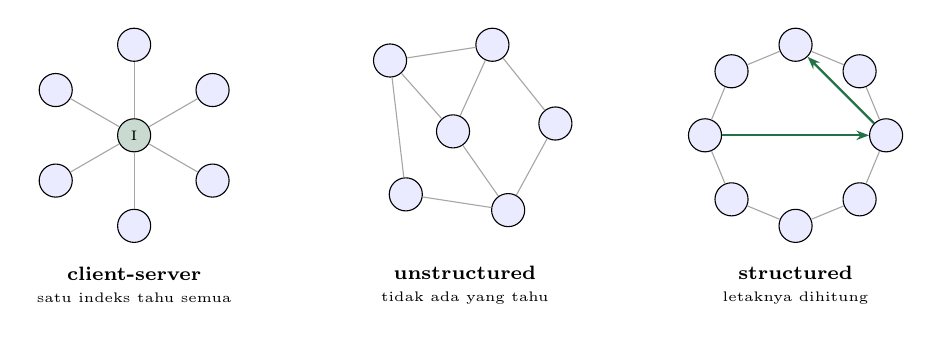
\begin{tikzpicture}[
    simpul/.style={circle, draw, minimum size=0.42cm, inner sep=0pt,
      font=\tiny, fill=blue!8},
    utama/.style={simpul, fill=praditagreen!25},
    garis/.style={thin, gray!70},
    judul/.style={font=\scriptsize\bfseries, align=center}
  ]
    \begin{scope}[shift={(0,0)}]
      \node[utama] (i) at (0,0) {I};
      \foreach \sudut in {30,90,150,210,270,330} {
        \node[simpul] (k\sudut) at (\sudut:1.15cm) {};
        \draw[garis] (i) -- (k\sudut);
      }
      \node[judul] at (0,-1.9) {client-server\\
        {\tiny\mdseries satu indeks tahu semua}};
    \end{scope}
    \begin{scope}[shift={(4.2,0)}]
      \node[simpul] (a) at (-0.95,0.95) {};
      \node[simpul] (b) at (0.35,1.15) {};
      \node[simpul] (c) at (1.15,0.15) {};
      \node[simpul] (d) at (0.55,-0.95) {};
      \node[simpul] (e) at (-0.75,-0.75) {};
      \node[simpul] (f) at (-0.15,0.05) {};
      \draw[garis] (a) -- (b);
      \draw[garis] (b) -- (c);
      \draw[garis] (c) -- (d);
      \draw[garis] (d) -- (e);
      \draw[garis] (e) -- (a);
      \draw[garis] (f) -- (b);
      \draw[garis] (f) -- (d);
      \draw[garis] (f) -- (a);
      \node[judul] at (0,-1.9) {unstructured\\
        {\tiny\mdseries tidak ada yang tahu}};
    \end{scope}
    \begin{scope}[shift={(8.4,0)}]
      \foreach \nomor/\sudut in {0/90,1/45,2/0,3/315,4/270,5/225,6/180,7/135} {
        \node[simpul] (c\nomor) at (\sudut:1.15cm) {};
      }
      \draw[garis] (c0) -- (c1);
      \draw[garis] (c1) -- (c2);
      \draw[garis] (c2) -- (c3);
      \draw[garis] (c3) -- (c4);
      \draw[garis] (c4) -- (c5);
      \draw[garis] (c5) -- (c6);
      \draw[garis] (c6) -- (c7);
      \draw[garis] (c7) -- (c0);
      \draw[-{Stealth[length=1.6mm]}, thick, praditagreen] (c6) -- (c2);
      \draw[-{Stealth[length=1.6mm]}, thick, praditagreen] (c2) -- (c0);
      \node[judul] at (0,-1.9) {structured\\
        {\tiny\mdseries letaknya dihitung}};
    \end{scope}
  \end{tikzpicture}}

  \vspace{8pt}
  {\small Yang membedakan bukan bentuk gambarnya, melainkan siapa yang
  mengetahui letak sebuah kunci.}
\end{frame}

\begin{frame}{{\Large Cara Ketiganya Menemukan Kunci}}
  \vspace{8pt}
  \begin{itemize}\small
    \item Client-server: seluruh kunci dititipkan kepada satu \textit{node}
          indeks. Peminta bertanya sekali, lalu dijawab.
    \item \textit{Unstructured}: kunci disebar acak dan letaknya tidak dicatat
          siapa pun. Pertanyaan disebar ke seluruh \textit{neighbor}, lalu
          diteruskan sampai batas empat \textit{hop}.
    \item \textit{Structured}: letak kunci dihitung dari hash namanya.
          Setiap \textit{node} menyimpan daftar pendek berisi \textit{node}
          untuk beberapa jarak berbeda, dan pertanyaan dioper ke yang terjauh
          tetapi belum melewati sasarannya.
  \end{itemize}

\end{frame}

\begin{frame}{{\Large Susunan Pertama: \textit{Centralized Index}}}
  \vspace{10pt}
  \begin{itemize}\small
    \item Analoginya mencari buku di asrama. Cara pertama, seorang penjaga
          memegang daftar siapa meminjam buku apa, lalu semua penghuni bertanya
          kepadanya.
    \item Seluruh kunci dititipkan kepada satu \textit{node} saja, yaitu
          \textit{node} bernomor nol, dan \textit{node} itu disebut indeks.
    \item \textit{Node} lain tidak menyimpan apa pun dan tidak saling
          mengenal, sehingga satu-satunya jalan adalah bertanya kepada indeks.
    \item Bentuk ini sama dengan client-server pada Bab 1, dan dipakai Napster
          untuk daftar \textit{file}.
  \end{itemize}

  \vspace{10pt}
  {\small Ketiga susunan dibahas berurutan, mulai dari yang paling sederhana
  ini.}
\end{frame}

\begin{frame}[fragile]{{\Large \textit{Centralized Index}: Metode \texttt{cari}}}
  \vspace{4pt}
\begin{lstlisting}[style=PythonStyle]
def cari(self, nomor_peminta: int, kunci: str):
  peminta = self.simpul[nomor_peminta]
  nilai = peminta.ambil(kunci)
  if nilai is not None:
    return jaringan.LookupResult(kunci, nilai, 0, 0)
  # satu pesan berangkat, satu pesan kembali
  indeks = self.simpul[NOMOR_INDEKS]
  nilai = indeks.ambil(kunci)
  return jaringan.LookupResult(kunci, nilai, 2, 1)
\end{lstlisting}
  \vspace{4pt}
  {\small Ongkosnya tetap dua pesan dan satu \textit{hop}, berapa pun jumlah
  \textit{node}-nya. Pesan pertama pertanyaan dari peminta kepada indeks, pesan
  kedua jawaban indeks kepada peminta, dan \textit{hop}-nya satu sebab
  pertanyaan itu hanya menyeberangi satu sambungan.}
\end{frame}

\begin{frame}{{\Large \textit{Centralized Index} pada Sistem Nyata}}
  \vspace{8pt}
  \centering
  \small
  \begin{tabularx}{0.95\textwidth}{|l|X|X|}
    \hline
    \textbf{Sistem} & \textbf{Letak indeks} & \textbf{Ketika indeks mati} \\
    \hline
    Napster & Server pusat menyimpan daftar \textit{file} seluruh pemakai & \textit{Lookup} berhenti sama sekali \\
    \hline
    BitTorrent & \textit{Tracker} menjawab dengan daftar \textit{node} pemegang \textit{file} & Unduhan yang berjalan bertahan, unduhan baru tidak \\
    \hline
    Contoh bab ini & \textit{Node} nol menyimpan seluruh 26 kunci kurs & Nol dari 200 \textit{lookup} terjawab \\
    \hline
  \end{tabularx}

  \vspace{8pt}
  {\small BitTorrent kemudian menambah jalan kedua, yaitu Distributed Hash
  Table berdasarkan Kademlia.}
\end{frame}

\begin{frame}{{\Large Susunan Kedua: \textit{Query Flooding}}}
  \vspace{2pt}
  \begin{columns}[c]
    \begin{column}{0.54\textwidth}
      \gambarkolom[0.64\textheight]{%
      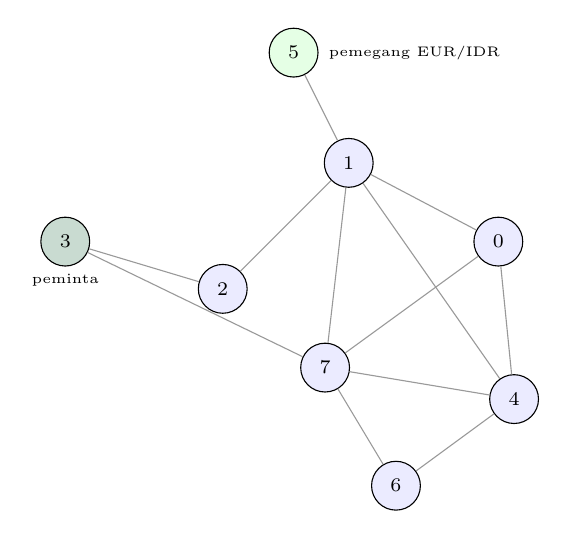
\begin{tikzpicture}[
        simpul/.style={circle, draw, minimum size=0.62cm, inner sep=0pt,
          font=\scriptsize, fill=blue!8},
        garis/.style={thin, gray!80},
        ket/.style={font=\tiny, inner sep=1.5pt}
      ]
        \node[simpul, fill=praditagreen!25] (n3) at (-1.5,1.0) {3};
        \node[simpul] (n2) at (0.5,0.4) {2};
        \node[simpul] (n1) at (2.1,2.0) {1};
        \node[simpul, fill=green!10] (n5) at (1.4,3.4) {5};
        \node[simpul] (n0) at (4.0,1.0) {0};
        \node[simpul] (n7) at (1.8,-0.6) {7};
        \node[simpul] (n4) at (4.2,-1.0) {4};
        \node[simpul] (n6) at (2.7,-2.1) {6};
        \draw[garis] (n0) -- (n1);
        \draw[garis] (n0) -- (n4);
        \draw[garis] (n0) -- (n7);
        \draw[garis] (n1) -- (n2);
        \draw[garis] (n1) -- (n4);
        \draw[garis] (n1) -- (n5);
        \draw[garis] (n1) -- (n7);
        \draw[garis] (n2) -- (n3);
        \draw[garis] (n3) -- (n7);
        \draw[garis] (n4) -- (n6);
        \draw[garis] (n4) -- (n7);
        \draw[garis] (n6) -- (n7);
        \node[ket, below=1pt of n3] {peminta};
        \node[ket, right=2pt of n5] {pemegang EUR/IDR};
      \end{tikzpicture}}
    \end{column}
    \begin{column}{0.44\textwidth}
      \vspace{14pt}
      \begin{itemize}\small
        \item Analoginya cara kedua di asrama, yaitu bertanya kepada teman
              sekamar, lalu diteruskan kepada teman mereka.
        \item Delapan \textit{node}, dua belas sambungan acak.
        \item Pertanyaan disebar sampai batas empat \textit{hop}, yaitu Time
              To Live pada Gnutella.
        \item \textit{Node} 5 hanya punya satu \textit{neighbor}.
      \end{itemize}
    \end{column}
  \end{columns}
\end{frame}

\begin{frame}[fragile]{{\Large Inti \textit{Query Flooding}}}
  \vspace{4pt}
\begin{lstlisting}[style=PythonStyle]
for tujuan in self.simpul[nomor].tetangga:
  if tujuan == pengirim:      # tidak kembali ke pengirim
    continue
  pesan += 1
  if tujuan in terlihat or not self.simpul[tujuan].hidup:
    continue                  # pertanyaan berulang dibuang
  terlihat.add(tujuan)
  temuan = self.simpul[tujuan].ambil(kunci)
  antrean.append((tujuan, nomor, jarak + 1))
\end{lstlisting}
  \vspace{4pt}
  {\small Penyebarannya tidak berhenti walaupun kuncinya sudah ketemu, sebab
  tidak ada \textit{node} yang tahu \textit{lookup} itu sudah selesai.}
\end{frame}

\begin{frame}{{\Large Susunan Ketiga: \textit{Identifier Ring}}}
  \vspace{8pt}
  \begin{itemize}\small
    \item Analoginya cara ketiga di asrama, yaitu seluruh penghuni
          menyepakati bahwa buku berawalan huruf tertentu selalu dititipkan di
          kamar bernomor tertentu, sehingga tidak ada yang perlu ditanya.
    \item Letak kunci dapat dihitung tanpa \textit{ring}, yaitu pengenal
          kunci dibagi jumlah \textit{node}, lalu sisanya menjadi nomor
          pemiliknya.
    \item Pembaginya adalah jumlah \textit{node}, sehingga satu \textit{node}
          yang bergabung mengubah pembagi itu dari delapan menjadi sembilan.
    \item Contohnya \texttt{USD/IDR} yang pengenalnya 40796. Dibagi delapan
          sisanya 4, dibagi sembilan sisanya 8, sehingga kuncinya harus pindah
          dari \textit{node} 4 ke \textit{node} 8.
  \end{itemize}

  \vspace{10pt}
  {\small Hal serupa terjadi pada hampir seluruh kunci lainnya, sehingga satu
  \textit{node} yang bergabung memindahkan hampir seluruh data.}
\end{frame}

\begin{frame}{{\Large Yang Ditawarkan \textit{Ring}}}
  \vspace{10pt}
  \begin{itemize}\small
    \item Pada \textit{ring}, yang berpindah hanya kunci di dalam busur milik
          \textit{node} baru. Sifat itu disebut \textit{consistent hashing}.
  \end{itemize}

  \vspace{10pt}
  \centering
  \small
  \begin{tabularx}{0.92\textwidth}{|X|l|l|}
    \hline
    \textbf{Kunci berpindah pemilik} & \textbf{Sisa bagi} & \textbf{\textit{Ring}} \\
    \hline
    8 menjadi 9 \textit{node} & 26 dari 26 & 1 dari 26 \\
    \hline
    16 menjadi 17 \textit{node} & 24 dari 26 & 2 dari 26 \\
    \hline
  \end{tabularx}

  \vspace{6pt}
  \raggedright
  {\small Setiap kunci yang berpindah berarti satu pemindahan data antar
  \textit{node}.}
\end{frame}

\begin{frame}{{\Large \textit{Identifier Ring}}}
  \vspace{2pt}
  \centering
  \resizebox{!}{0.66\textheight}{%
  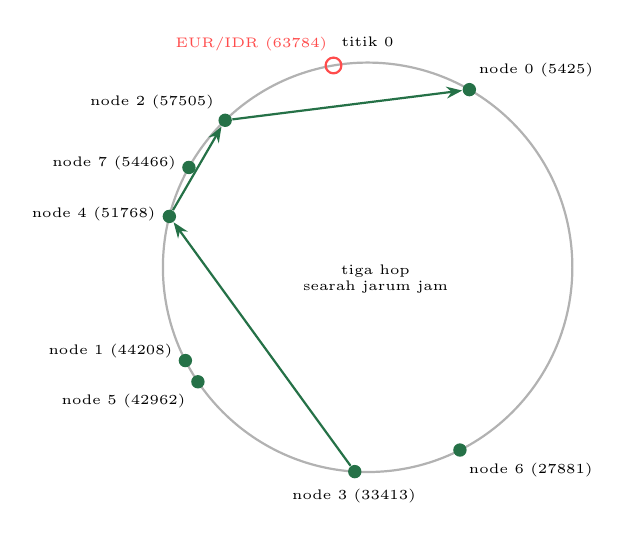
\begin{tikzpicture}[
    titik/.style={circle, fill=praditagreen, minimum size=0.17cm,
      inner sep=0pt},
    nama/.style={font=\tiny, inner sep=1.5pt},
    panah/.style={-{Stealth[length=2mm]}, thick, praditagreen}
  ]
    \draw[gray!60, thick] (0,0) circle (2.6cm);
    \node[font=\tiny, above] at (0,2.68) {titik 0};
    \node[titik] (s0) at (60.2:2.6cm) {};
    \node[titik] (s2) at (134.1:2.6cm) {};
    \node[titik] (s7) at (150.8:2.6cm) {};
    \node[titik] (s4) at (165.6:2.6cm) {};
    \node[titik] (s1) at (207.1:2.6cm) {};
    \node[titik] (s5) at (214.0:2.6cm) {};
    \node[titik] (s3) at (266.4:2.6cm) {};
    \node[titik] (s6) at (296.8:2.6cm) {};
    \node[circle, draw=red!70, thick, minimum size=0.2cm, inner sep=0pt]
      at (99.6:2.6cm) {};
    \node[nama, anchor=south east, text=red!70] at (99.6:2.72cm)
      {EUR/IDR (63784)};
    \node[nama, anchor=south west] at (60.2:2.72cm) {node 0 (5425)};
    \node[nama, anchor=south east] at (134.1:2.72cm) {node 2 (57505)};
    \node[nama, anchor=east] at (150.8:2.72cm) {node 7 (54466)};
    \node[nama, anchor=east] at (165.6:2.72cm) {node 4 (51768)};
    \node[nama, anchor=east, yshift=5pt] at (207.1:2.72cm) {node 1 (44208)};
    \node[nama, anchor=east, yshift=-5pt] at (214.0:2.72cm) {node 5 (42962)};
    \node[nama, anchor=north] at (266.4:2.76cm) {node 3 (33413)};
    \node[nama, anchor=north west] at (296.8:2.72cm) {node 6 (27881)};
    \draw[panah] (s3) -- (s4);
    \draw[panah] (s4) -- (s2);
    \draw[panah] (s2) -- (s0);
    \node[font=\tiny, align=center] at (0.1,-0.15)
      {tiga hop\\ searah jarum jam};
  \end{tikzpicture}}

  \vspace{4pt}
  {\small Kunci pada titik 63784 dititipkan kepada penerusnya, yaitu \textit{node} 0.}
\end{frame}

\begin{frame}[fragile]{{\Large Contoh Perhitungan Titiknya}}
  \vspace{4pt}
\begin{lstlisting}[language=bash]
python -c "import cincin; print(cincin.pengenal_dari('EUR/IDR'))"
# Keluarannya: 63784
python -c "import cincin; print(cincin.pengenal_dari('simpul-0'))"
# Keluarannya: 5425
\end{lstlisting}

  \vspace{4pt}
  \begin{enumerate}\small
    \item Nama di-hash dengan SHA-1, lalu hasilnya diambil sisa baginya terhadap
          65536, sehingga jatuh pada salah satu titik ruang enam belas bit.
    \item Nama kunci dan nama \textit{node} memakai fungsi yang sama, sehingga
          \texttt{EUR/IDR} jatuh di titik 63784 dan \texttt{simpul-0} di titik
          5425.
    \item Pemiliknya dicari searah jarum jam, yaitu \textit{node} pertama yang
          titiknya tidak kurang dari 63784.
    \item Titik \textit{node} terbesar hanya 57505, sehingga pencariannya
          melewati titik 0 lalu berhenti di \textit{node} 0 pada titik 5425.
  \end{enumerate}
\end{frame}

\begin{frame}{{\Large Mengapa Harus Melompat}}
  \vspace{6pt}
  \begin{itemize}\small
    \item Letak kunci dapat dihitung, tetapi tidak satu \textit{node} pun
          menyimpan daftar seluruh \textit{node}.
    \item Yang pasti diketahui setiap \textit{node} hanya penerusnya, yaitu
          \textit{node} terdekat searah jarum jam.
    \item Mengoper lewat penerus saja memang sampai, tetapi pada delapan
          \textit{node} satu \textit{lookup} dapat menempuh tujuh \textit{hop}.
    \item \textit{Finger table} menyediakan jalan pintas, dan jalan pintas
          terjauh melompati separuh \textit{ring}.
  \end{itemize}

  \vspace{8pt}
  \centering
  \small
  \begin{tabularx}{0.9\textwidth}{|X|l|l|}
    \hline
    \textbf{Dua ratus \textit{lookup}} & \textbf{Penerus saja} & \textbf{\textit{Finger table}} \\
    \hline
    \textit{Hop} median & 4 & 2 \\
    \hline
    \textit{Hop} terbesar & 7 & 4 \\
    \hline
    Pesan median & 8 & 4 \\
    \hline
  \end{tabularx}
\end{frame}

\begin{frame}{{\Large Apa Itu \textit{Finger Table}}}
  \vspace{10pt}
  \begin{itemize}\small
    \item Buku alamat kecil di dalam setiap \textit{node}, berisi enam belas
          baris.
    \item Setiap baris menyimpan satu \textit{node} yang pantas dihubungi untuk
          satu jarak tertentu.
    \item Jaraknya berlipat dua, yaitu 1, 2, 4, 8, dan seterusnya sampai separuh
          \textit{ring}.
    \item Tidak memuat daftar seluruh \textit{node}, sehingga tetap enam belas
          baris walaupun jaringannya berisi sejuta \textit{node}.
  \end{itemize}

  \vspace{10pt}
  {\small Tanpa jalan pintas itu, satu \textit{lookup} rata-rata menempuh separuh
  jumlah \textit{node}, yaitu sekitar lima ratus ribu \textit{hop} pada sejuta
  \textit{node}. Dengan jalan pintas, cukup sekitar dua puluh \textit{hop}.}
\end{frame}

\begin{frame}[fragile]{{\Large \textit{Finger Table} dan Penelusurannya}}
  \vspace{4pt}
  \centering
  \scriptsize
  \begin{tabularx}{0.92\textwidth}{|l|l|l|X|}
    \hline
    \textbf{\textit{Finger} ke-$i$} & \textbf{Titik dicari} & \textbf{Penerusnya} & \textbf{Titik penerus} \\
    \hline
    0 sampai 13 & 33414 sampai 41605 & \textit{node} 5 & 42962 \\
    \hline
    14 & 49797 & \textit{node} 4 & 51768 \\
    \hline
    15 & 645 & \textit{node} 0 & 5425 \\
    \hline
  \end{tabularx}

  \vspace{4pt}
\begin{lstlisting}[style=PythonStyle]
while lompatan < BATAS_LOMPATAN:
  penerus = self.penerus_hidup(sekarang)
  if di_antara(sasaran, sekarang.pengenal, penerus.pengenal):
    nilai = penerus.ambil(kunci)
    return jaringan.LookupResult(kunci, nilai, lompatan * 2, lompatan)
  sekarang = self.jari_terdekat(sekarang, sasaran) or penerus
\end{lstlisting}
\end{frame}

\begin{frame}{{\Large Tujuh Kelas yang Dipakai}}
  \vspace{6pt}
  \centering
  \scriptsize
  \begin{tabularx}{0.97\textwidth}{|l|X|}
    \hline
    \textbf{Kelas} & \textbf{Perannya} \\
    \hline
    \texttt{Network} & Kerangka bersama, menyerahkan \texttt{susun} dan \texttt{cari} kepada turunannya \\
    \hline
    \texttt{Node} & Satu \textit{node} beserta titipan kunci dan daftar \textit{neighbor} \\
    \hline
    \texttt{LookupResult} & Catatan satu \textit{lookup}: nilai, jumlah pesan, jumlah \textit{hop} \\
    \hline
    \texttt{IndexNetwork} & Client-server, seluruh kunci pada satu \textit{node} indeks \\
    \hline
    \texttt{FloodingNetwork} & \textit{Unstructured}, pertanyaan disebar ke seluruh \textit{neighbor} \\
    \hline
    \texttt{RingNetwork} & \textit{Structured}, letak kunci dihitung pada \textit{identifier ring} \\
    \hline
    \texttt{RingNode} & Turunan \texttt{Node} yang membawa titik \textit{ring} dan \textit{finger table} \\
    \hline
  \end{tabularx}
\end{frame}

\begin{frame}{{\Large \textit{Class Diagram}: Satu Kerangka}}
  \vspace{4pt}
  \begin{center}
    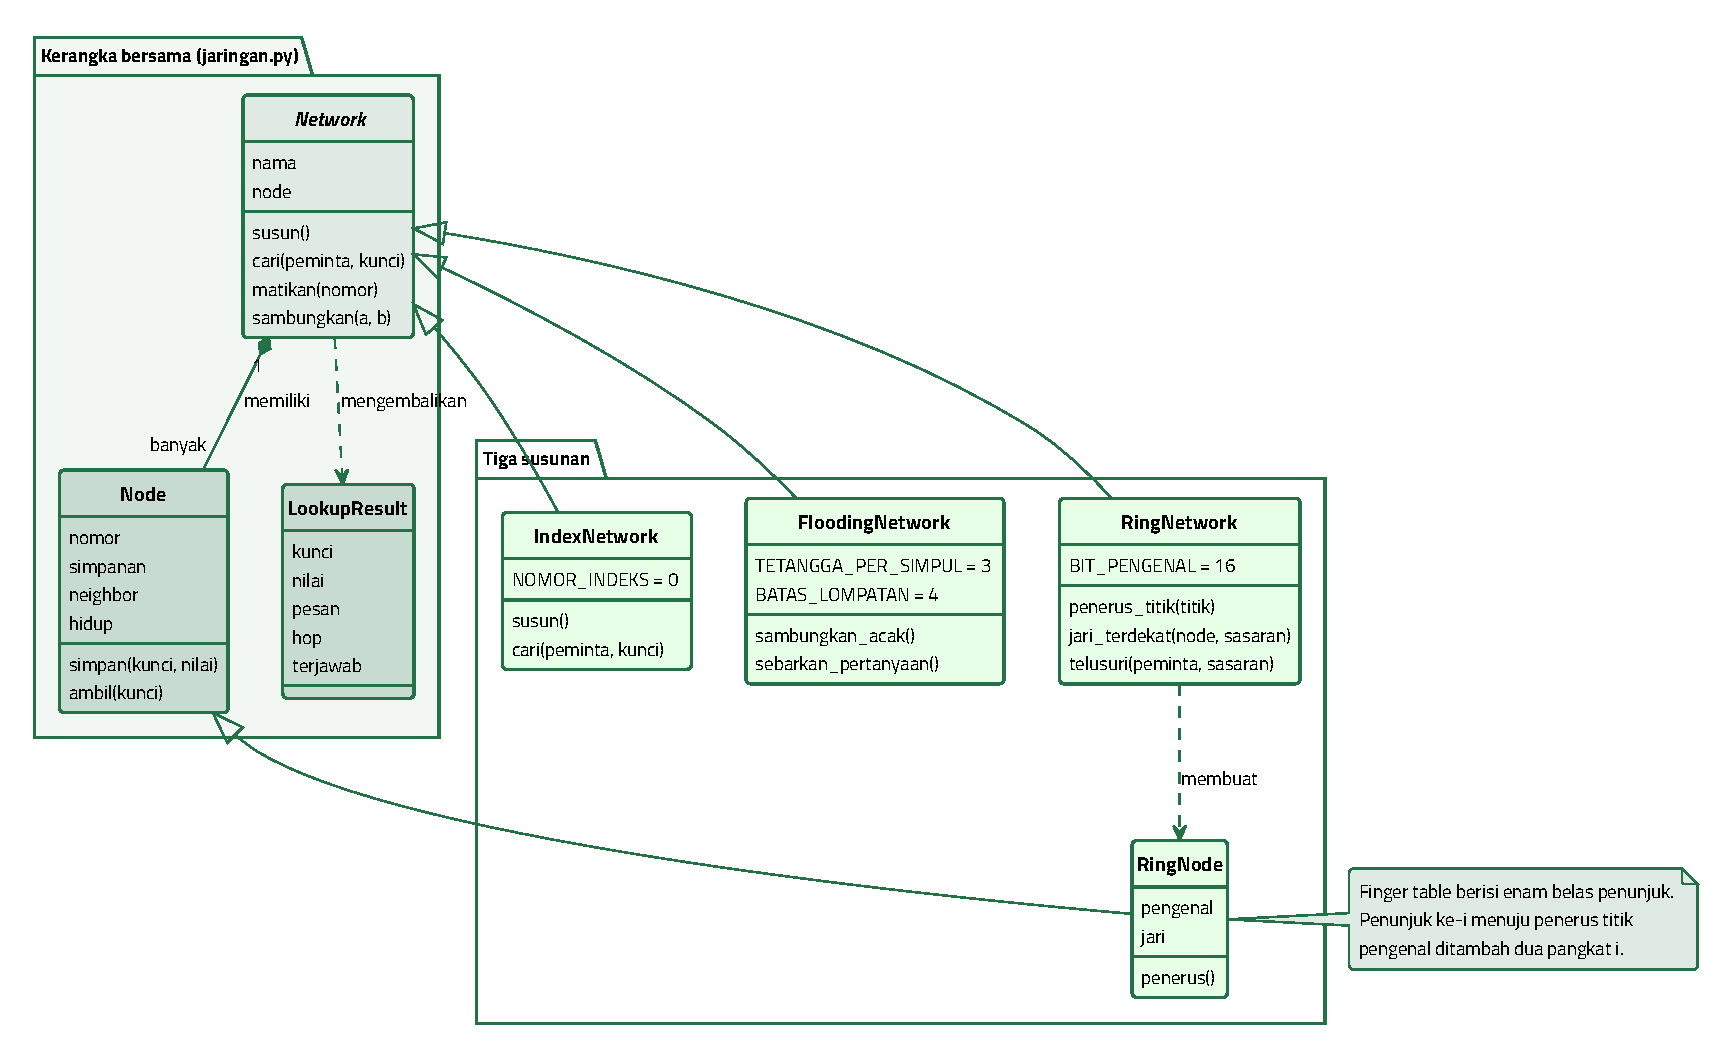
\includegraphics[width=\textwidth, height=0.74\textheight,
      keepaspectratio]{kelas-p2p.pdf}
  \end{center}
\end{frame}

\begin{frame}{{\Large Penjelasan \textit{Class Diagram}}}
  \vspace{10pt}
  \begin{itemize}\small
    \item Kerangkanya menyiapkan \textit{node} dan pengacak dengan
          \textit{seed} tetap.
    \item Ketiga turunannya hanya menimpa dua metode, yaitu \texttt{susun}
          yang menitipkan kunci dan \texttt{cari} yang menemukannya kembali.
    \item \textit{Finger table} hanya dimiliki \texttt{RingNode}, sedangkan dua
          susunan lain memakai \texttt{Node} apa adanya.
    \item Sisanya sama persis, yaitu 26 kunci kurs, daftar peminta, dan
          \textit{seed} pengacaknya.
  \end{itemize}

  \vspace{10pt}
  {\small Karena yang berbeda hanya kedua metode itu, selisih pesan dan
  \textit{hop} antara ketiga susunan benar-benar berasal dari cara menitipkan
  dan cara mencari, bukan dari bahan yang berbeda.}
\end{frame}

\begin{frame}{{\Large Jalur \textit{Unstructured}}}
  \vspace{6pt}
  \begin{center}
    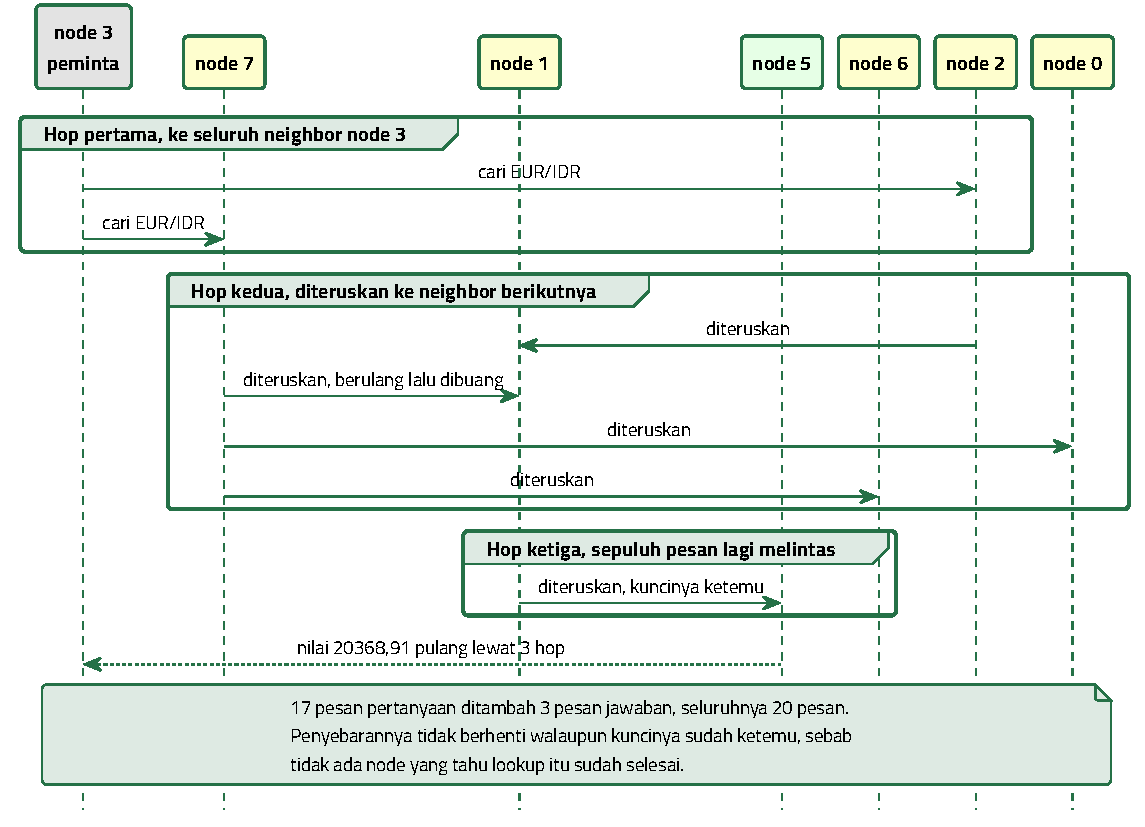
\includegraphics[width=0.94\textwidth, height=0.62\textheight,
      keepaspectratio]{sekuens-p2p-unstructured.pdf}
  \end{center}
  \vspace{2pt}
  {\small Disebar ke seluruh \textit{neighbor}, seluruhnya 20 pesan.}
\end{frame}

\begin{frame}{{\Large Jalur \textit{Structured}}}
  \vspace{6pt}
  \begin{center}
    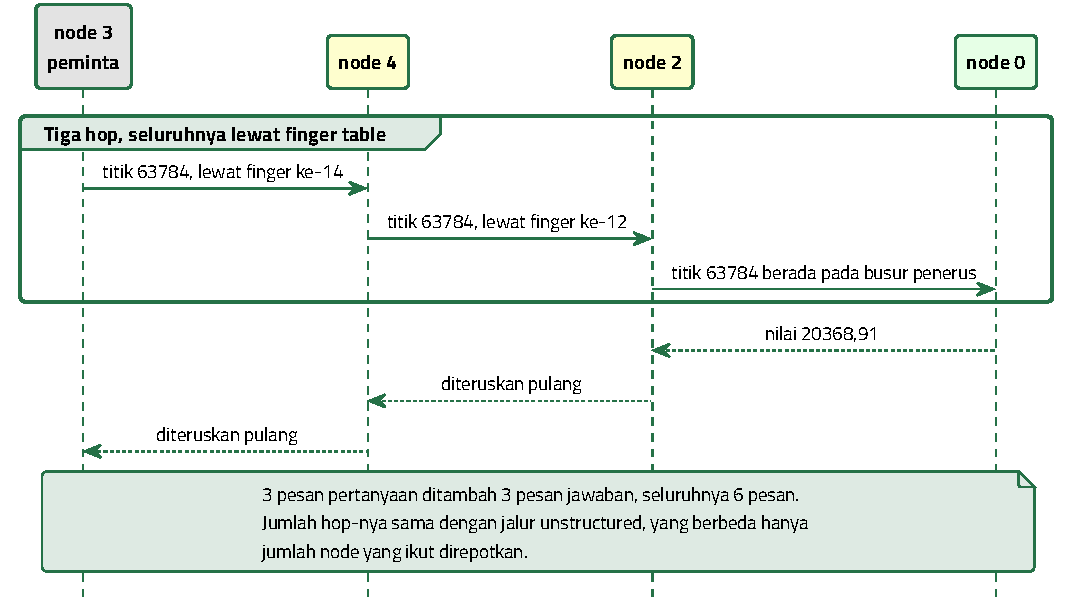
\includegraphics[width=0.80\textwidth, height=0.62\textheight,
      keepaspectratio]{sekuens-p2p-structured.pdf}
  \end{center}
  \vspace{2pt}
  {\small Kunci, peminta, dan jumlah \textit{hop}-nya sama. Yang berbeda jumlah
  \textit{node} yang ikut direpotkan, yaitu 6 pesan melawan 20 pesan.}
\end{frame}

\begin{frame}{{\Large Kasus: Pemeliharaan Dua Jam}}
  \vspace{8pt}
  \begin{enumerate}\small
    \item Sebuah tim membangun layanan kurs internal untuk delapan kantor
          cabang, memakai satu \textit{centralized index}.
    \item Tabel kursnya disimpan pada satu mesin di kantor pusat, sebab cara
          itu paling mudah diawasi.
    \item Pada suatu Jumat sore, mesin tersebut dimatikan untuk pemeliharaan
          yang dijadwalkan dua jam.
    \item Seluruh cabang seketika kehilangan kurs, padahal masing-masing sudah
          membacanya berkali-kali.
  \end{enumerate}

  \vspace{8pt}
  {\small Tidak satu cabang pun menyimpan salinannya, sebab susunannya memang
  tidak menuntut hal itu.}
\end{frame}

\begin{frame}{{\Large Hasil: \textit{Lookup Cost}}}
  \vspace{6pt}
  \centering
  \small
  \begin{tabularx}{0.95\textwidth}{|X|l|l|l|}
    \hline
    \textbf{Yang diukur} & \textbf{Client-server} & \textbf{Tak \textit{structured}} & \textbf{\textit{Structured}} \\
    \hline
    Pesan median & 2 & 19 & 4 \\
    \hline
    Pesan persentil ke-95 & 2 & 20 & 6 \\
    \hline
    Pesan terbesar & 2 & 20 & 8 \\
    \hline
    \textit{Hop} median & 1 & 2 & 2 \\
    \hline
    \textit{Hop} terbesar & 1 & 3 & 4 \\
    \hline
    Sisi jaringan & 7 & 12 & 13 \\
    \hline
  \end{tabularx}

  \vspace{6pt}
  {\small Sambungannya hampir sama banyak, sehingga selisih pesannya benar-benar
  berasal dari cara mencari. Dua ratus \textit{lookup}, delapan \textit{node}.}
\end{frame}

\begin{frame}{{\Large Hasil: \textit{Failure Resilience}}}
  \vspace{6pt}
  \centering
  \small
  \begin{tabularx}{0.95\textwidth}{|X|l|l|l|}
    \hline
    \textbf{Yang diukur} & \textbf{Client-server} & \textbf{Tak \textit{structured}} & \textbf{\textit{Structured}} \\
    \hline
    Seluruh \textit{node} hidup & 200 dari 200 & 200 dari 200 & 200 dari 200 \\
    \hline
    \textit{Node} 0 mati & 0,0 persen & 94,0 persen & 86,0 persen \\
    \hline
    Rata-rata satu \textit{node} mati & 87,5 persen & 83,5 persen & 87,9 persen \\
    \hline
    Terburuk satu \textit{node} mati & 0,0 persen & 55,2 persen & 71,5 persen \\
    \hline
    Kunci pada \textit{node} terburuk & 26 & 4 & 7 \\
    \hline
  \end{tabularx}

  \vspace{6pt}
  {\small Menurut rata-rata, client-server mengungguli susunan \textit{unstructured}.
  Baris terburuklah yang memperlihatkan titik kegagalan tunggalnya.}
\end{frame}

\begin{frame}{{\Large Hasil: \textit{Message Scalability}}}
  \vspace{6pt}
  \centering
  \small
  \begin{tabularx}{0.95\textwidth}{|X|l|l|l|}
    \hline
    \textbf{Yang diukur} & \textbf{Client-server} & \textbf{Tak \textit{structured}} & \textbf{\textit{Structured}} \\
    \hline
    Pesan median 8 \textit{node} & 2 & 19 & 4 \\
    \hline
    Pesan median 16 \textit{node} & 2 & 35 & 6 \\
    \hline
    Pertumbuhan pesan & 1,00 kali & 1,84 kali & 1,50 kali \\
    \hline
    \textit{Hop} median 16 \textit{node} & 1 & 2 & 3 \\
    \hline
    Terjawab pada 16 \textit{node} & 200 & 199 & 200 \\
    \hline
  \end{tabularx}

  \vspace{6pt}
  {\small Pembandingnya 2,00 kali bila ongkos tumbuh sebanding dengan jumlah
  \textit{node}, dan 1,33 kali bila sebanding dengan logaritmanya.}
\end{frame}

\begin{frame}{{\Large Kapan Masing-Masing Dipakai}}
  \vspace{8pt}
  \centering
  \small
  \begin{tabularx}{0.96\textwidth}{|l|X|X|}
    \hline
    \textbf{Susunan} & \textbf{Dipakai ketika} & \textbf{Harga yang dibayar} \\
    \hline
    Client-server & Jaringan dimiliki satu pihak, keanggotaan jarang berubah & Nol persen \textit{lookup} terjawab saat indeksnya mati \\
    \hline
    \textit{Unstructured} & Tidak ada yang berwenang memegang indeks & 19 pesan per \textit{lookup}, tumbuh 1,84 kali \\
    \hline
    \textit{Structured} & Jaringan besar, keanggotaan berubah terus & \textit{Finger table} beserta pemeliharaannya \\
    \hline
  \end{tabularx}

  \vspace{8pt}
  \raggedright
  {\small Napster memakai indeks terpusat, Gnutella memakai penyebaran sesudah
  Napster dihentikan, dan Amazon Dynamo memakai \textit{ring}. BitTorrent
  memakai dua sekaligus, yaitu \textit{tracker} beserta \textit{distributed hash
  table}.}
\end{frame}

\begin{frame}{{\Large Ringkasan}}
  \vspace{10pt}
  \begin{itemize}\small
    \item Kedudukan yang sama membawa satu pekerjaan baru, yaitu menemukan data
          tanpa ada \textit{node} yang tahu seluruh isi jaringan.
    \item Indeks terpusat membayar dua pesan, susunan \textit{unstructured} 19 pesan,
          susunan \textit{structured} empat pesan.
    \item Rata-rata ketahanan ketiganya hampir sama, sehingga yang dibaca
          adalah giliran terburuknya, yaitu nol persen melawan 55,2 dan 71,5.
    \item Penggandaan \textit{node} menumbuhkan pesan 1,84 kali pada susunan tak
          \textit{structured}, dan 1,50 kali pada susunan \textit{structured}.
  \end{itemize}

  \vspace{10pt}
  {\small Pesan utamanya, ketiadaan pusat dibayar dengan pekerjaan \textit{lookup},
  dan besarnya ditentukan oleh struktur yang bersedia dipelihara.}
\end{frame}

\begin{frame}[fragile]{{\Large Persiapan Latihan}}
  \vspace{5pt}
\begin{lstlisting}[language=bash]
bash sources/siapkan_venv.sh
source .venv/bin/activate
cd sources/chapter07
python susunan.py daftar
# Kunci kurs terdaftar : 26 (18 September 2026)
python susunan.py cari cincin EUR/IDR
# Jumlah hop      : 3
\end{lstlisting}

  \vspace{6pt}
  {\small Bab ini hanya memakai pustaka standar Python, sehingga tidak ada
  pemasangan tambahan. Langkah lengkap, tabel contoh, dan lembar isian ada di
  modul Bab 7, yang menjadi rujukan utama latihan ini.}
\end{frame}

\begin{frame}[fragile]{{\Large Latihan 1: \textit{Lookup Cost}}}
  \vspace{3pt}
\begin{lstlisting}[language=bash]
python ukur_pencarian.py
# Susunan unstructured: Pesan median 19.0  Hop median 2.0
# Susunan structured  : Pesan median  4.0  Hop median 2.0
python susunan.py cari tetangga EUR/IDR
# Jumlah pesan    : 20
python susunan.py cari cincin EUR/IDR
# Jumlah pesan    : 6
\end{lstlisting}

  \vspace{3pt}
  \begin{enumerate}\small
    \item Catat keenam angka sebaran untuk setiap susunan.
    \item Tunjukkan baris pada \texttt{tetangga.py} yang membuang pertanyaan
          berulang.
    \item Ubah \texttt{BATAS\_LOMPATAN} dari empat menjadi dua, lalu catat
          pesan dan \textit{lookup} yang terjawab.
  \end{enumerate}

  \vspace{3pt}
  {\small Pertanyaan: mengapa sebaran pesan susunan \textit{unstructured} hampir
  rata, sedangkan susunan \textit{structured} melebar dari empat sampai delapan?}
\end{frame}

\begin{frame}[fragile]{{\Large Latihan 2: \textit{Failure Resilience}}}
  \vspace{3pt}
\begin{lstlisting}[language=bash]
python uji_ketahanan.py
# Terburuk client-server : 0.0 persen
# Terburuk unstructured  : 55.2 persen (node 1)
# Terburuk structured    : 71.5 persen (node 6)
\end{lstlisting}

  \vspace{3pt}
  \begin{enumerate}\small
    \item Catat kelima baris hasil untuk setiap susunan.
    \item Bandingkan baris rata-rata dengan baris terburuk pada susunan
          client-server.
    \item Jalankan \texttt{python tetangga.py} dan \texttt{python cincin.py},
          lalu cari \textit{node} yang paling rapuh.
  \end{enumerate}

  \vspace{3pt}
  {\small Pertanyaan: rata-rata client-server justru paling tinggi. Mengapa
  angka itu menyesatkan, dan baris mana yang seharusnya dibaca?}
\end{frame}

\begin{frame}[fragile]{{\Large Latihan 3: \textit{Message Scalability}}}
  \vspace{3pt}
\begin{lstlisting}[language=bash]
python ukur_penskalaan.py
# Pertumbuhan jumlah node : 2.00 kali
# Pertumbuhan unstructured: 1.84 kali
# Pertumbuhan structured  : 1.50 kali
python ukur_pencarian.py 32
# Susunan unstructured: Pesan median 52.0  terjawab 172 dari 200
\end{lstlisting}

  \vspace{3pt}
  \begin{enumerate}\small
    \item Catat kedua angka pembanding pada kepala laporannya.
    \item Catat pertumbuhan pesan ketiga susunan beserta \textit{hop} mediannya.
    \item Catat pesan median pada 32 \textit{node} beserta \textit{lookup} yang tidak
          terjawab.
  \end{enumerate}

  \vspace{3pt}
  {\small Pertanyaan: dengan menggabungkan hasil ketiga latihan, susunan mana
  yang dipakai untuk jaringan berisi sejuta \textit{node}?}
\end{frame}

\end{document}
